%%%%%%%%%%%%%%%%%%%%%%%%%%%%%%%%%%%%%%%%%%%%%%%%%%%%%%%%%%%%%%%%%%%%%%%%%%%%%%%%%%%%%%%%%%%%%%%%%%%%%%%%%%%%%%%%%%%%%%%%%%%%%%%%%%%%%%%%%%%%%%%%%%%%%%%%%%%%%%%%%%%%%%%%%%%%%%%%%%%%%%%%%%%%%%%%%%%%%%%%
% Table generated by Excel2LaTeX from sheet 'C1EX1'
\chapter{Graphique n°2}
\begin{longtable}{|r|r|}
	\hline
	\multicolumn{1}{|c|}{$x$} & \multicolumn{1}{c|}{$y$} \\
	\hline
	16     & 20  \\
	\hline
	18     & 24  \\
	\hline
	23     & 28  \\
	\hline
	24     & 22  \\
	\hline
	26     & 32  \\
	\hline
	28     & 32  \\
	\hline
	29     & 28  \\
	\hline
	31     & 36  \\
	\hline
	32     & 41  \\
	\hline
	34     & 41  \\
	\hline
\end{longtable}%


\begin{figure}[H]
	\centering
	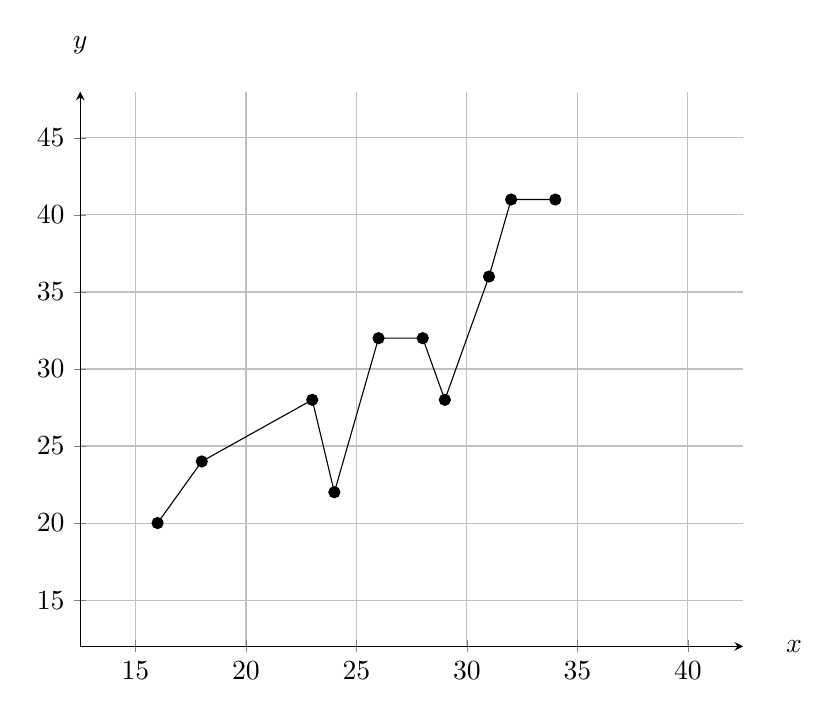
\begin{tikzpicture}
		\begin{axis}[
			xlabel={$x$},
			ylabel={$y$},
			legend pos=north east,
			grid=major,
			xmin=15, xmax=40,
			ymin=15, ymax=45,
			axis x line=middle, 
			axis y line=middle, 
			samples=1000, 
			xlabel = $x$, 
			ylabel=$y$,
			enlargelimits,
			xlabel style={at={(ticklabel* cs:1.05)}, anchor=west}, % Place le nom de l'axe x à droite de l'axe
			ylabel style={at={(ticklabel* cs:1.05)}, anchor=south}, % Place le nom de l'axe y au-dessus de l'axe
			width=10cm,
			]
			
			\addplot[mark=*] coordinates {
				(16,20)
				(18,24)
				(23,28)
				(24,22)
				(26,32)
				(28,32)
				(29,28)
				(31,36)
				(32,41)
				(34,41)
			};
			
			%\addplot[domain=15:40, line width=0.95pt]{1.116545*x+1.258177} node[pos=0.95, anchor=east]{$\text{1.116545}x+\text{1.258177}$};;
			
		\end{axis}
	\end{tikzpicture}
\end{figure}

% Define a custom style for STATA code



\begin{lstlisting}[style=stata, label={lst:stata}]
	*Calcul du coeffcient de corrélation entre x et y
	
	pwcorr x y, sig star(5)
	
	*Test de significativité
	
	gen t*=abs(0.8929)/sqrt((1-0.8929^2)/(_N-2))
	display t*
\end{lstlisting}

Le code ci-dessus permet d'obtenir les valeurs respectives du coefficient de corrélation (0,8929) pour un seuil de 5\% et de la statistique de Student ($t^*$=5,61). On compare ainsi cette valeur à $\displaystyle t_{10-2}^{5\%/2}$ ou $\displaystyle  t_{8}^{2.5\%}=2,306$. On peut remarquer que $\displaystyle t^*>t_{8}^{2.5\%}=2,306$; dès lors l'hypothèse H$_0$ est rejetée et H$_1$ est acceptée.

Les variables $x$ et $y$ évoluent par conséquent dans le même sens.

 \begin{figure}[h]
	\begin{center}
		\begin{tikzpicture}
			\begin{axis}[
				grid=both,
				xmin=0,
				xmax=6, 
				ymin=-4, 
				ymax=8, 
				axis x line=middle, 
				axis y line=middle, 
				samples=1000, 
				xlabel = $x$, 
				ylabel=$f(x)$,
				enlargelimits,
				xlabel style={at={(ticklabel* cs:1.05)}, anchor=west}, % Place le nom de l'axe x à droite de l'axe
				ylabel style={at={(ticklabel* cs:1.05)}, anchor=south}, % Place le nom de l'axe y au-dessus de l'axe
				width=15cm]
				
				%Dessiner graphique 1
				\addplot[domain=0:5, color=red, line width=.95pt]{abs(x*ln(x))} node[above]{$f(x)=|x\ln(x)|$};
				%Ajouter points
				\addplot[soldot, red] coordinates {(1/e,1/e)};
				\addplot[soldot, red] coordinates {(1,0)};
				%Tracer tangente
				\addplot[holdot, red] coordinates{(0,0)};
				\draw[<->, line width=1pt] (0.27,0.4) -- (0.47,0.4);
				%Dessiner graphique 2
				\addplot[domain=0:5, color=orange, line width=0.95pt]{x*ln(x)} node[pos=0.95,
				anchor=east]{$g(x)=x\ln(x)$};
				%Ajouter points
				\addplot[soldot, orange] coordinates {(1/e,-1/e)};
				%Tracer tangente
				\draw[<->, line width=1pt] (0.27,-0.4) -- (0.47,-0.4);
				\draw[<->, line width=1pt] (0.9,-0) -- (1.1,-0);
			\end{axis}
		\end{tikzpicture}
	\end{center}
	\caption{Graphique des fonctions $\displaystyle f(x)=\lvert x\ln(x) \rvert$ \& $\displaystyle g(x)=x\ln(x)$}
\end{figure}

Ce graphique met donc en évidence une relation symétrique avec l'axe des abscisses des fonctions $|x\ln(x)|$ et $x\ln(x)$ sur l'intervalle $]0;1[$ et une convexité de ces fonctions sur $\mathbb{R}^{*}_{+}-\{1\}$.